\documentclass{article}

\usepackage{graphicx}
\usepackage{tikz}
\usepackage{tikzsymbols}
\usetikzlibrary{calc,patterns,shapes.geometric}
\pagestyle{empty}
\usepackage[margin=0pt]{geometry}
\geometry{papersize={14in,12in}}

\def\centerarc[#1](#2)(#3:#4:#5){\draw[#1] ($(#2)+({#5*cos(#3)},{#5*sin(#3)})$) arc (#3:#4:#5);}

\begin{document}
	\begin{figure}
		\centering
		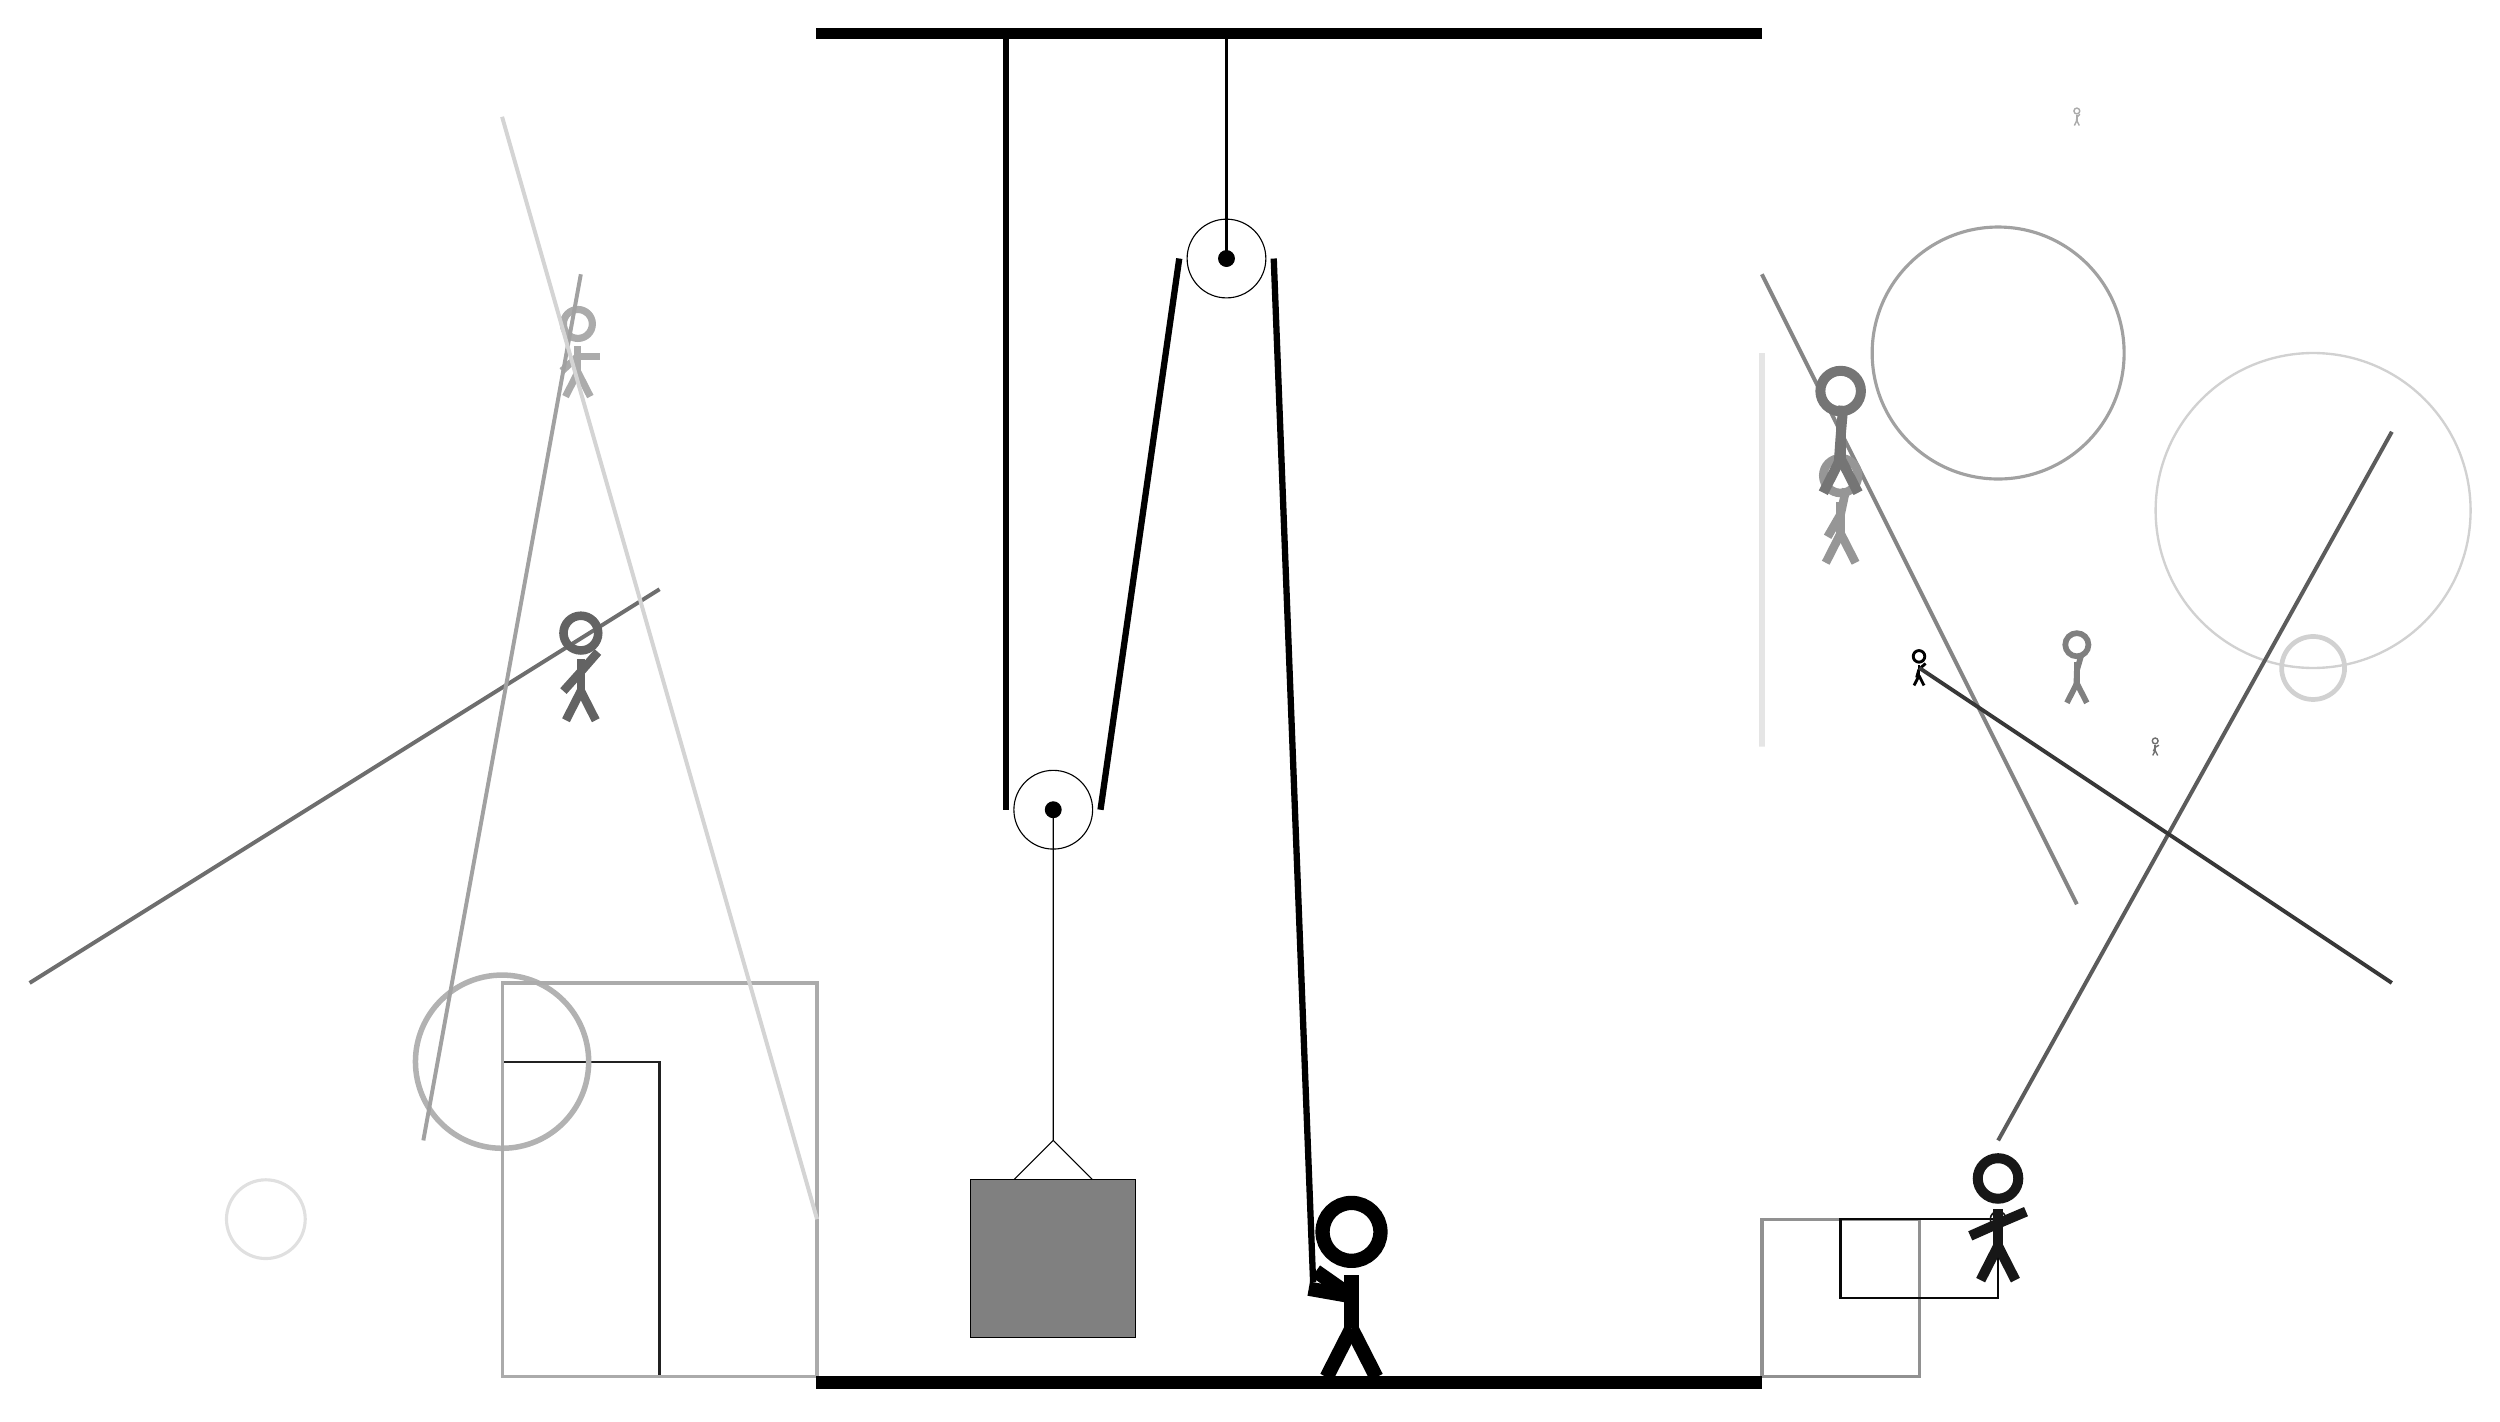
\begin{tikzpicture}
			%%%%% START %%%%%
			
			\draw[fill=black] (-2, 14) rectangle (10, 14.125);
			
			\draw (3.2, 11.2) circle (0.5);
			\draw[fill=black] (3.2, 11.2) circle (0.1);
			\draw[thick] (3.2, 11.2) -- (3.2, 14);
			
			\draw[line width=0.5mm, color=black!57](-4, 7) -- (-12, 2);
			
			\node[line width=0.2mm, color=black!50] at (14, 6) {\Strichmaxerl[4][88][74]};
			\node[line width=0.2mm, color=black!33] at (-5, 10) {\Strichmaxerl[5][43][0]};
			\draw [line width=0.3mm, color=black!18](17, 8) circle (2.0);
			\draw[line width=0.7mm, color=black!10] (10, 10) rectangle (10, 5);
			\draw[line width=0.3mm, color=black!87] (-4, 1) rectangle (-6, -3);
			
			\draw[line width=0.5mm, color=black!48](10, 11) -- (14, 3);
			\node[line width=0.5mm, color=black!100] at (12, 6) {\Strichmaxerl[2][74][41]};
			\node[line width=0.5mm, color=black!41] at (11, 8) {\Strichmaxerl[6][60][78]};
			\draw [line width=0.4mm, color=black!37](13, 10) circle (1.6);
			\draw [line width=0.4mm, color=black!64](15, 13) circle (0.0);
			\draw [line width=0.4mm, color=black!12](-9, -1) circle (0.5);
			\draw[line width=0.4mm, color=black!43] (10, -3) rectangle (12, -1);
			\draw[line width=0.3mm, color=black!97] (11, -2) rectangle (13, -1);
			\node[line width=0.7mm, color=black!61] at (-5, 6) {\Strichmaxerl[6][48][49]};
			\draw [line width=0.7mm, color=black!30](-6, 1) circle (1.1);
			\draw[line width=0.4mm, color=black!33] (-2, 2) rectangle (-6, -3);
			\draw [line width=0.6mm, color=black!18](17, 6) circle (0.4);
			\draw[line width=0.5mm, color=black!37](-5, 11) -- (-7, 0);
			\draw[line width=0.5mm, color=black!64](13, 0) -- (18, 9);
			\draw[line width=0.5mm, color=black!17](-2, -1) -- (-6, 13);
			
			\draw [line width=0.2mm, color=black!93](13, -1) circle (0.1);
			
			\node[line width=0.2mm, color=black!33] at (14, 13) {\Strichmaxerl[1][85][47]};
			\node[line width=0.6mm, color=black!56] at (15, 5) {\Strichmaxerl[1][65][30]};
			\node[line width=0.7mm, color=black!54] at (11, 9) {\Strichmaxerl[7][86][85]};
			\node[line width=0.4mm, color=black!91] at (13, -1) {\Strichmaxerl[7][24][23]};
			\draw[line width=0.5mm, color=black!78](12, 6) -- (18, 2);
			
			\draw (1, 4.2) circle (0.5);
			\draw[fill=black] (1, 4.2) circle (0.1);
			
			\draw (1, 4.2) -- (1, 0) -- (0.5, -0.5);
			\draw (1, 0) -- (1.5, -0.5);
			\draw[fill=black!50] (-0.05, -0.5) rectangle (2.05, -2.5);
			
			\draw[line width=0.8mm] (0.4, 14) -- (0.4, 4.2);
			\centerarc[line width=0.8mm](1, 4.2)(180:360:0.6);
			\draw[line width=0.8mm](1.6, 4.2) -- (2.6, 11.2);
			\centerarc[line width=0.8mm](3.2, 11.2)(0:180:0.6);
			\draw[line width=0.8mm](3.8, 11.2) -- (4.3, -1.8);
			
			\node at (4.7, -1.9) {\Strichmaxerl[10][-35][170]};
			
			\draw[fill=black] (-2, -3) rectangle (10, -3.15);
			
			%%%%% END %%%%%
		\end{tikzpicture}
	\end{figure}	
\end{document}